


\section{Research methodology}
%- Forschungsmethodik/Vorgehen
%   -- vorgehen mit beispiel der Forschungsfragen

The bachelor thesis aims to solve the issue whether the Rocchio relevance feedback algorithm is capable of satisfying all requirements or not.
To do so, the requirements a recommender system has to match will be defined.
Also there will be a distinction of various approaches to generate suggestions such as "content-based", "knowledge-based", etc.\\
In order to test a recommender system one will be built, based on Rocchio's information retrieval algorithm.
The implementation will be combined with an online-shop - even though the online shop will only concentrate on the core-component of presenting products.\\
A characteristic of this algorithm is the way it refines the set of recommendations every time a user gives more information about his preferences.\citep[p. 92]{lops:11}
The process of learning about the user can be both implicit, or explicit.
Learning based on implicit behaviour will be implemented in the first version.
Depending on the time schedule an alternative implementation with explicit user feedback is possible.\\

Software is much more than pure source-code.
As addition to every program a proper documentation is expected, as well a "tidied up" source-code that can be maintained easily.
For this reason the process of software-development has to be planned in-depth and documented accurately.


\subsection{Proceeding}
By the time the project is finished there will be two software-components.\\
First, a recommender-library which is capable of handling product-data and generating recommendation for any user based on his preceding (shopping-)behaviour.
Second, a online-shop that presents products and provides recommendations for products the user might like, based on the recommender-library.
As programming language for implementing the recommender-library Python has been chosen.
In order to make the library interoperable with other programming languages a web-API may be built.

\subsection{Documentation}
The theory of the code will be explained in a separate document with many examples to visualize the way the recommendation system works.
Additionally there will be a documentation based on python-sphinx which will be automatically generated out of source-code comments.


\subsection{Milestones}
The development of the recommender algorithm will be subdivided into stages.
These can be seen in figure~\ref{fig:softwaremilestones}.
Each of the steps has to be finished before the next can start.\\

\begin{figure}[h!]

    \centering

    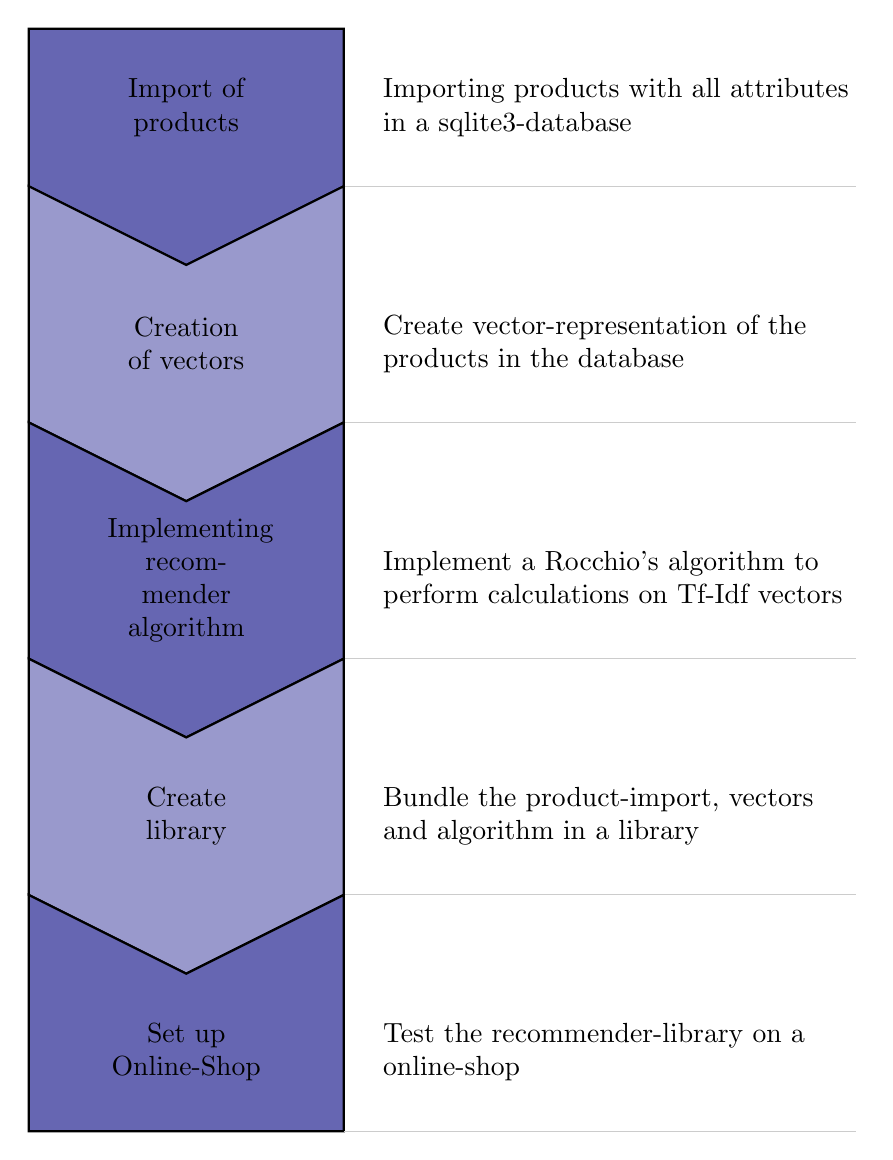
\begin{tikzpicture}

        \draw[thick,fill=Navy!60]
            (0,0)--(2,-1)--(4,0)--(4,2)--(0,2)--cycle;
        \node[text width=2cm,text centered,yshift=0] at (2,1) {Import of products};
        \node[text width=6cm,align=left,yshift=0] at (7.5,1) {Importing products with all attributes in a sqlite3-database};
        \draw[thin,Black!20,yshift=0] (4,0)--(10.5,0);

        \draw[thick,fill=Navy!40,yshift=-3cm]
            (0,0)--(2,-1)--(4,0)--(4,3)--(2,2)--(0,3)--cycle;
        \node[text width=2cm,text centered,yshift=-3cm] at (2,1) {Creation of vectors};
        \node[text width=6cm,align=left,yshift=-3cm] at (7.5,1) {Create vector-representation of the products in the database};
        \draw[thin,Black!20,yshift=-3cm] (4,0)--(10.5,0);

        \draw[thick,fill=Navy!60,yshift=-6cm]
            (0,0)--(2,-1)--(4,0)--(4,3)--(2,2)--(0,3)--cycle;
        \node[text width=2cm,text centered,yshift=-6cm] at (2,1) {Implementing recommender algorithm};
        \node[text width=6cm,align=left,yshift=-6cm] at (7.5,1) {Implement a Rocchio's algorithm to perform calculations on Tf-Idf vectors};
        \draw[thin,Black!20,yshift=-6cm] (4,0)--(10.5,0);

        \draw[thick,fill=Navy!40,yshift=-9cm]
            (0,0)--(2,-1)--(4,0)--(4,3)--(2,2)--(0,3)--cycle;
        \node[text width=2cm,text centered,yshift=-9cm] at (2,1) {Create library};
        \node[text width=6cm,align=left,yshift=-9cm] at (7.5,1) {Bundle the product-import, vectors and algorithm in a library};
        \draw[thin,Black!20,yshift=-9cm] (4,0)--(10.5,0);

        \draw[thick,fill=Navy!60,yshift=-12cm]
            (0,0)--(4,0)--(4,3)--(2,2)--(0,3)--cycle;
        \node[text width=2cm,text centered,yshift=-12cm]at (2,1) {Set up Online-Shop};
        \node[text width=6cm,align=left,yshift=-12cm] at (7.5,1) {Test the recommender-library on a online-shop};
        \draw[thin,Black!20,yshift=-12cm] (4,0)--(10.5,0);

    \end{tikzpicture}

    \caption[Software Milestones]{software milestones}
    \label{fig:softwaremilestones}
\end{figure}


\FloatBarrier

